\documentclass[11pt,a4paper]{article}

% ============ PACKAGES ============
\usepackage[utf8]{inputenc}
\usepackage[T1]{fontenc}
\usepackage{geometry}
\geometry{margin=1in}
\usepackage{graphicx}
\usepackage{booktabs}
\usepackage{array}
\usepackage{multirow}
\usepackage{amsmath,amssymb}
\usepackage{hyperref}
\usepackage{xcolor}
\usepackage{float}
\usepackage{caption}
\usepackage{subcaption}
\usepackage[numbers,sort&compress]{natbib}
\usepackage{algorithm}
\usepackage{algpseudocode}
\usepackage{enumitem}
\usepackage{tcolorbox}
\usepackage{fancyhdr}
\usepackage{diagbox}
\usepackage{lastpage}

% ============ SETTINGS ============
\hypersetup{
    colorlinks=true,
    linkcolor=blue,
    citecolor=blue,
    urlcolor=blue
}

\pagestyle{fancy}
\fancyhf{}
\rhead{Research Progress Report}
\lhead{Relaxed Equivariance in GNNs}
\rfoot{Page \thepage\ of \pageref{LastPage}}

% Custom commands
\newcommand{\todo}[1]{\textcolor{red}{\textbf{[TODO: #1]}}}
\newcommand{\inprogress}[1]{\textcolor{orange}{\textbf{[IN PROGRESS: #1]}}}
\newcommand{\completed}[1]{\textcolor{green!60!black}{\checkmark\ #1}}

% ============ DOCUMENT ============
\begin{document}

% ============ TITLE PAGE ============
\begin{titlepage}
    \centering
    \vspace*{2cm}
    
    {\LARGE\textbf{Research Progress Report}}\\[0.5cm]
    {\Large Probabilistic Graphical Models }\\[2cm]
    
    {\Huge\textbf{Relaxed Equivariance via Multitask Learning}}\\[0.3cm]
    {\Huge\textbf{with Layer-Depth-Adaptive Equivariant}}\\[0.3cm]
    {\Huge\textbf{Loss Rates in Graph Neural Networks}}\\[2cm]
    
    % {\Large\textbf{Project Group 1}}\\[0.5cm]
    {\large Ahmed Alhassan \quad Manyara Baraka }\\[2cm]
    
    \begin{tcolorbox}[colback=blue!5!white,colframe=blue!75!black,title=\textbf{Progress Summary}]
    \begin{itemize}[leftmargin=*]
        \item \textbf{Total Experiments Completed:} 142 of 200+ planned
        \item \textbf{Phases Completed:} Phase 1 (GCN), Phase 2 (GIN/GraphSAGE)
        \item \textbf{Phases In Progress:} Depth Study (59\%), Ablation Study (56\%)
        \item \textbf{Key Finding:} Architecture selection dominates; GIN baseline achieves $R^2=0.838$, outperforming all equivariance-regularized variants
    \end{itemize}
    \end{tcolorbox}
    
    \vfill
    
    {\large\textbf{GitHub:} \url{https://github.com/[repository]}}\\[0.5cm]
    {\large Last Updated: \today}
    
\end{titlepage}

% ============ TABLE OF CONTENTS ============
\tableofcontents
\newpage

% ============ SECTION 1: EXECUTIVE SUMMARY ============
\section{Executive Summary}

This progress report documents our research on \textbf{relaxed equivariance via multitask learning} in Graph Neural Networks (GNNs). The core innovation treats equivariance as a soft, learnable constraint rather than a hard architectural requirement, with constraint strength varying by layer depth according to the formulation:
\begin{equation}
    \mathcal{L}_{\text{total}} = \mathcal{L}_{\text{task}} + \sum_{l=1}^{L} \alpha_l \cdot \mathcal{L}_{\text{eq}}^{(l)}
\end{equation}

\subsection{Key Accomplishments}
\begin{enumerate}
    \item \textbf{Completed 142 experiments} across three GNN architectures (GCN, GIN, GraphSAGE) with five scheduling strategies on ZINC12k dataset
    \item \textbf{Discovered architecture-dependent benefits}: Equivariance regularization improves GCN (+2.8\% $R^2$) but \textit{hurts} GIN ($-18\%$ degradation)
    \item \textbf{Validated learnable scheduling}: Learnable $\alpha_l$ parameters achieve best performance for GCN with lowest variance across seeds
    \item \textbf{Established strong baselines}: GIN baseline ($R^2=0.838$) significantly outperforms all other configurations
\end{enumerate}

\subsection{Current Status}

\begin{table}[H]
\centering
\caption{Experiment Completion Status}
\label{tab:status}
\begin{tabular}{llccc}
\toprule
\textbf{Phase} & \textbf{Description} & \textbf{Completed} & \textbf{Total} & \textbf{Status} \\
\midrule
Phase 1 & GCN Scheduling Study & 54 & 54 & \completed{Complete} \\
Phase 2 & Architecture Comparison & 50 & 50 & \completed{Complete} \\
Ablation & $\alpha_0 \times \beta$ Grid & 22 & 39 & \inprogress{56\%} \\
Depth & Network Depth Study & 16 & 27 & \inprogress{59\%} \\
Phase 3 & QM9 3D Dataset & 9 & 30+ & \inprogress{Paused} \\
\midrule
\textbf{Total} & & \textbf{142} & \textbf{200+} & \textbf{71\%} \\
\bottomrule
\end{tabular}
\end{table}

% ============ SECTION 2: INTRODUCTION ============
\section{Introduction}

\subsection{Problem Statement}

Equivariance under group actions (permutations, rotations, reflections) is a powerful inductive bias in deep learning for structured data \cite{bronstein2021geometric}. Models that respect data symmetries---including Graph Neural Networks (GNNs) and equivariant transformers---can generalize better, require fewer samples, and more accurately represent underlying structure. However, enforcing \textit{strict} equivariance constrains the hypothesis space and can prevent fitting phenomena where symmetry should be broken.

Recent works highlight the need for \textbf{relaxation}---controlling the strength and form of equivariance via auxiliary objectives or learnable parameters \cite{elhag2024remul, vanderouderaa2023layerwise, hofgard2024relaxed}. Our research investigates depth-scheduled, multitask equivariant losses in GNNs to improve their flexibility, empirical performance, and interpretability.

\subsection{Research Questions}

This project addresses four primary research questions:

\begin{enumerate}
    \item \textbf{RQ1:} How do different scheduling strategies (constant, exponential, linear, learnable) affect task performance and equivariance satisfaction?
    
    \item \textbf{RQ2:} Does the benefit of relaxed equivariance depend on the base architecture (GCN vs. GIN vs. GraphSAGE)?
    
    \item \textbf{RQ3:} What is the optimal depth profile for equivariance constraints---should early layers be more strictly equivariant than later layers?
    
    \item \textbf{RQ4:} Can learnable layer-wise weights $\alpha_l$ automatically discover optimal equivariance schedules?
\end{enumerate}

\subsection{Contributions}

Our contributions to date include:

\begin{enumerate}
    \item \textbf{Comprehensive empirical study} of depth-adaptive equivariance across 142 experiments with rigorous multi-seed evaluation
    
    \item \textbf{Novel finding} that equivariance regularization benefits depend strongly on architecture expressivity---less expressive models (GCN) benefit while more expressive models (GIN) are harmed
    
    \item \textbf{Validation of learnable scheduling} as the most robust approach for GCN, achieving lowest variance across random seeds
    
    \item \textbf{Reproducible experimental framework} with comprehensive logging, configuration management, and statistical analysis
    
    \item \textbf{Open-source implementation} integrating with PyTorch Geometric and Weights \& Biases
\end{enumerate}

% ============ SECTION 3: RELATED WORK ============
\section{Related Work}

\subsection{Geometric Deep Learning and Equivariance}

Bronstein et al. \cite{bronstein2021geometric} provide the foundational framework for geometric deep learning, unifying approaches across grids, groups, graphs, geodesics, and gauges. The key insight is that neural network architectures should respect the symmetries inherent in the data domain.

For graphs, permutation equivariance is the fundamental symmetry: reordering nodes should not change the network output (for graph-level tasks) or should permute accordingly (for node-level tasks). Classical GNN architectures---GCN \cite{kipf2017gcn}, GIN \cite{xu2019gin}, GraphSAGE \cite{hamilton2017graphsage}---achieve permutation equivariance through aggregation operations that are inherently order-invariant.

\subsection{Strict vs. Relaxed Equivariance}

For 3D molecular and physical systems, geometric equivariance (SO(3), SE(3), E(3)) becomes important. Architectures like SchNet \cite{schutt2018schnet}, PaiNN \cite{schutt2021painn}, EGNN \cite{satorras2021egnn}, and Equiformer \cite{liao2023equiformer} enforce strict geometric equivariance through carefully designed operations.

However, strict equivariance has limitations:
\begin{itemize}
    \item \textbf{Computational cost}: Tensor product operations and spherical harmonics are expensive
    \item \textbf{Reduced expressivity}: Hard constraints limit the function class
    \item \textbf{Imperfect symmetries}: Real-world data often has approximate or broken symmetries
\end{itemize}

\subsection{Relaxed Equivariance Frameworks}

Recent work has explored relaxing equivariance constraints:

\textbf{REMUL} \cite{elhag2024remul} proposes treating equivariance as a multitask learning objective, achieving 10$\times$ faster inference and 2.5$\times$ faster training compared to strictly equivariant baselines while maintaining competitive performance.

\textbf{Layer-wise Equivariance Learning} \cite{vanderouderaa2023layerwise} uses Bayesian marginal likelihood optimization via Laplace approximations to automatically discover optimal equivariance strengths at each layer, primarily demonstrated on CNNs.

\textbf{Relaxed E(3)-Equivariance} \cite{hofgard2024relaxed} introduces non-scalar weights enabling controlled symmetry breaking in 3D geometric networks.

\textbf{Approximate Equivariance} \cite{wang2022approximate} studies networks for imperfectly symmetric dynamics, showing that controlled relaxation can improve generalization.

Our work extends these ideas by:
\begin{enumerate}
    \item Systematically comparing multiple scheduling strategies on GNNs
    \item Evaluating across architectures with different expressivity levels
    \item Using learnable parameters to discover optimal depth profiles
\end{enumerate}

% ============ SECTION 4: METHODOLOGY ============
\section{Methodology}

\subsection{Problem Formulation}

Given a graph $G = (V, E)$ with node features $\mathbf{X} \in \mathbb{R}^{|V| \times d}$ and edge features $\mathbf{E}$, we train a GNN $f_\theta: G \rightarrow \mathbb{R}$ for graph-level regression. The standard training objective minimizes task loss:
\begin{equation}
    \mathcal{L}_{\text{task}} = \frac{1}{N} \sum_{i=1}^{N} \left( f_\theta(G_i) - y_i \right)^2
\end{equation}

We augment this with layer-wise equivariance penalties:
\begin{equation}
    \mathcal{L}_{\text{total}} = \mathcal{L}_{\text{task}} + \sum_{l=1}^{L} \alpha_l \cdot \mathcal{L}_{\text{eq}}^{(l)}
    \label{eq:total_loss}
\end{equation}

where $\alpha_l \geq 0$ controls the equivariance constraint strength at layer $l$.

\subsection{Equivariance Loss Computation}

For a symmetry group $\mathcal{G}$ (e.g., permutation group $S_n$), the equivariance loss at layer $l$ measures how well the layer representation commutes with group actions:
\begin{equation}
    \mathcal{L}_{\text{eq}}^{(l)} = \mathbb{E}_{g \sim \mathcal{G}} \left\| f^{(l)}(g \cdot \mathbf{X}) - g \cdot f^{(l)}(\mathbf{X}) \right\|^2
\end{equation}

In practice, we approximate this expectation by sampling random group elements:
\begin{equation}
    \mathcal{L}_{\text{eq}}^{(l)} \approx \frac{1}{K} \sum_{k=1}^{K} \left\| f^{(l)}(g_k \cdot \mathbf{X}) - g_k \cdot f^{(l)}(\mathbf{X}) \right\|^2
\end{equation}

For permutation equivariance, $g_k$ are random node permutations applied to the graph.

\subsection{Scheduling Strategies}

We implement and evaluate five scheduling strategies for the layer-wise weights $\alpha_l$:

\begin{enumerate}
    \item \textbf{Baseline} ($\alpha_l = 0$): No equivariance regularization---standard GNN training
    
    \item \textbf{Constant} ($\alpha_l = \alpha_0$): Uniform equivariance weight across all layers
    
    \item \textbf{Exponential Decay}: 
    \begin{equation}
        \alpha_l = \alpha_0 \cdot \exp(-\beta \cdot l)
    \end{equation}
    Strong equivariance in early layers, relaxing in deeper layers
    
    \item \textbf{Linear Decay}:
    \begin{equation}
        \alpha_l = \max(0, \alpha_0 - \gamma \cdot l)
    \end{equation}
    Linearly decreasing equivariance constraint with depth
    
    \item \textbf{Learnable}: 
    \begin{equation}
        \alpha_l = \text{softplus}(\theta_l)
    \end{equation}
    where $\theta_l$ are learnable parameters optimized jointly with network weights
\end{enumerate}

\subsection{Model Architectures}

We evaluate three GNN architectures with different expressivity levels:

\textbf{Graph Convolutional Network (GCN)} \cite{kipf2017gcn}:
\begin{equation}
    \mathbf{h}_v^{(l+1)} = \sigma\left( \sum_{u \in \mathcal{N}(v) \cup \{v\}} \frac{1}{\sqrt{d_u d_v}} \mathbf{W}^{(l)} \mathbf{h}_u^{(l)} \right)
\end{equation}

\textbf{Graph Isomorphism Network (GIN)} \cite{xu2019gin}:
\begin{equation}
    \mathbf{h}_v^{(l+1)} = \text{MLP}^{(l)}\left( (1 + \epsilon^{(l)}) \cdot \mathbf{h}_v^{(l)} + \sum_{u \in \mathcal{N}(v)} \mathbf{h}_u^{(l)} \right)
\end{equation}

\textbf{GraphSAGE} \cite{hamilton2017graphsage}:
\begin{equation}
    \mathbf{h}_v^{(l+1)} = \sigma\left( \mathbf{W}^{(l)} \cdot \text{CONCAT}\left( \mathbf{h}_v^{(l)}, \text{AGG}(\{\mathbf{h}_u^{(l)} : u \in \mathcal{N}(v)\}) \right) \right)
\end{equation}

GIN is theoretically the most expressive (as powerful as the Weisfeiler-Lehman test), followed by GraphSAGE, then GCN.

\subsection{Implementation Details}

Our implementation uses:
\begin{itemize}
    \item \textbf{Framework}: PyTorch 2.0+ with PyTorch Geometric
    \item \textbf{Optimization}: Adam optimizer with cosine annealing learning rate schedule
    \item \textbf{Regularization}: Dropout (0.5), early stopping (patience=20)
    \item \textbf{Logging}: Weights \& Biases for experiment tracking
    \item \textbf{Reproducibility}: 5 random seeds per configuration (42, 123, 456, 789, 1000)
\end{itemize}

% ============ SECTION 5: EXPERIMENTAL SETUP ============
\section{Experimental Setup}

\subsection{Dataset: ZINC12k}

We use the ZINC12k molecular dataset for graph-level regression:

\begin{table}[H]
\centering
\caption{ZINC12k Dataset Statistics}
\label{tab:zinc_stats}
\begin{tabular}{ll}
\toprule
\textbf{Property} & \textbf{Value} \\
\midrule
Training graphs & 10,000 \\
Validation graphs & 1,000 \\
Test graphs & 1,000 \\
Average nodes per graph & 23.2 \\
Average edges per graph & 49.8 \\
Node feature dimension & 39 (one-hot atom type + degree) \\
Task & Constrained solubility regression \\
Metric & Mean Absolute Error (MAE), $R^2$ \\
\bottomrule
\end{tabular}
\end{table}

\subsection{Training Configuration}

\begin{table}[H]
\centering
\caption{Training Hyperparameters}
\label{tab:hyperparams}
\begin{tabular}{ll}
\toprule
\textbf{Hyperparameter} & \textbf{Value} \\
\midrule
Hidden dimension & 64 \\
Number of layers & 4 (default) \\
Dropout rate & 0.5 \\
Learning rate & 0.001 \\
LR scheduler & Cosine annealing \\
Batch size & 32 \\
Maximum epochs & 300 \\
Early stopping patience & 20 \\
Optimizer & Adam ($\beta_1=0.9, \beta_2=0.999$) \\
Number of seeds & 5 \\
\midrule
\multicolumn{2}{l}{\textit{Equivariance Loss Parameters}} \\
$\alpha_0$ (initial strength) & 1.0 (default) \\
$\beta$ (exponential decay) & 0.1 (default) \\
$\gamma$ (linear decay) & 0.1 (default) \\
Symmetry group & Permutation ($S_n$) \\
Samples per batch & 3 \\
\bottomrule
\end{tabular}
\end{table}

\subsection{Experiment Phases}

Our experimental campaign consists of five phases:

\begin{enumerate}
    \item \textbf{Phase 1: GCN Scheduling Study} (Complete)
    \begin{itemize}
        \item Compare 5 scheduling strategies on GCN architecture
        \item 5 seeds $\times$ 5 schedules = 25 base experiments
        \item Additional runs for validation = 54 total
    \end{itemize}
    
    \item \textbf{Phase 2: Architecture Comparison} (Complete)
    \begin{itemize}
        \item Extend to GIN and GraphSAGE architectures
        \item 2 models $\times$ 5 schedules $\times$ 5 seeds = 50 experiments
    \end{itemize}
    
    \item \textbf{Ablation Study} (In Progress: 56\%)
    \begin{itemize}
        \item Grid search over $\alpha_0 \in \{0.0, 0.1, 0.5, 1.0\}$ and $\beta \in \{0.0, 0.1, 0.3, 0.5\}$
        \item 13 configurations $\times$ 3 seeds = 39 experiments
        \item 22 completed, 17 remaining
    \end{itemize}
    
    \item \textbf{Depth Study} (In Progress: 59\%)
    \begin{itemize}
        \item Evaluate depths $\in \{4, 8, 16\}$ with different schedules
        \item 3 depths $\times$ 3 schedules $\times$ 3 seeds = 27 experiments
        \item 16 completed, 11 remaining
    \end{itemize}
    
    \item \textbf{Phase 3: QM9 3D Dataset} (Paused)
    \begin{itemize}
        \item Extend to 3D molecular data with SO(3)/E(3) symmetries
        \item 9 experiments completed, paused for computational reasons
    \end{itemize}
\end{enumerate}

% ============ SECTION 6: RESULTS ============
\section{Results}

We present results from 142 completed experiments across all phases. All metrics are reported as mean $\pm$ standard deviation across random seeds.

\subsection{Phase 1: GCN Scheduling Comparison}

\begin{table}[H]
\centering
\caption{Phase 1: GCN Results by Scheduling Strategy (ZINC12k, 5 seeds)}
\label{tab:phase1}
\begin{tabular}{lccccc}
\toprule
\textbf{Schedule} & \textbf{Test MAE} $\downarrow$ & \textbf{Test $R^2$} $\uparrow$ & \textbf{Val MAE} & \textbf{Epochs} & \textbf{Best Seed} \\
\midrule
Baseline & $0.591 \pm 0.022$ & $0.649 \pm 0.013$ & $0.584 \pm 0.022$ & 264.2 & 789 \\
Constant & $0.582 \pm 0.016$ & $0.660 \pm 0.014$ & $0.574 \pm 0.018$ & 270.6 & 789 \\
Exponential & $0.578 \pm 0.009$ & $0.666 \pm 0.008$ & $0.569 \pm 0.011$ & 265.3 & 1000 \\
Linear & $0.577 \pm 0.011$ & $0.665 \pm 0.008$ & $0.568 \pm 0.009$ & 275.2 & 456 \\
\textbf{Learnable} & $\mathbf{0.571 \pm 0.010}$ & $\mathbf{0.667 \pm 0.007}$ & $\mathbf{0.561 \pm 0.009}$ & 285.2 & 1000 \\
\bottomrule
\end{tabular}
\end{table}

\textbf{Key Findings:}
\begin{itemize}
    \item \textbf{Learnable scheduling achieves best performance} ($R^2 = 0.667$) with \textbf{lowest variance} ($\pm 0.007$)
    \item All equivariance-regularized variants outperform baseline (+1.6\% to +2.8\% relative $R^2$ improvement)
    \item Exponential and linear decay perform similarly, suggesting gradual relaxation is beneficial
    \item Learnable schedule requires slightly more epochs (285 vs 264) but converges to better solutions
\end{itemize}

\begin{figure}[H]
    \centering
    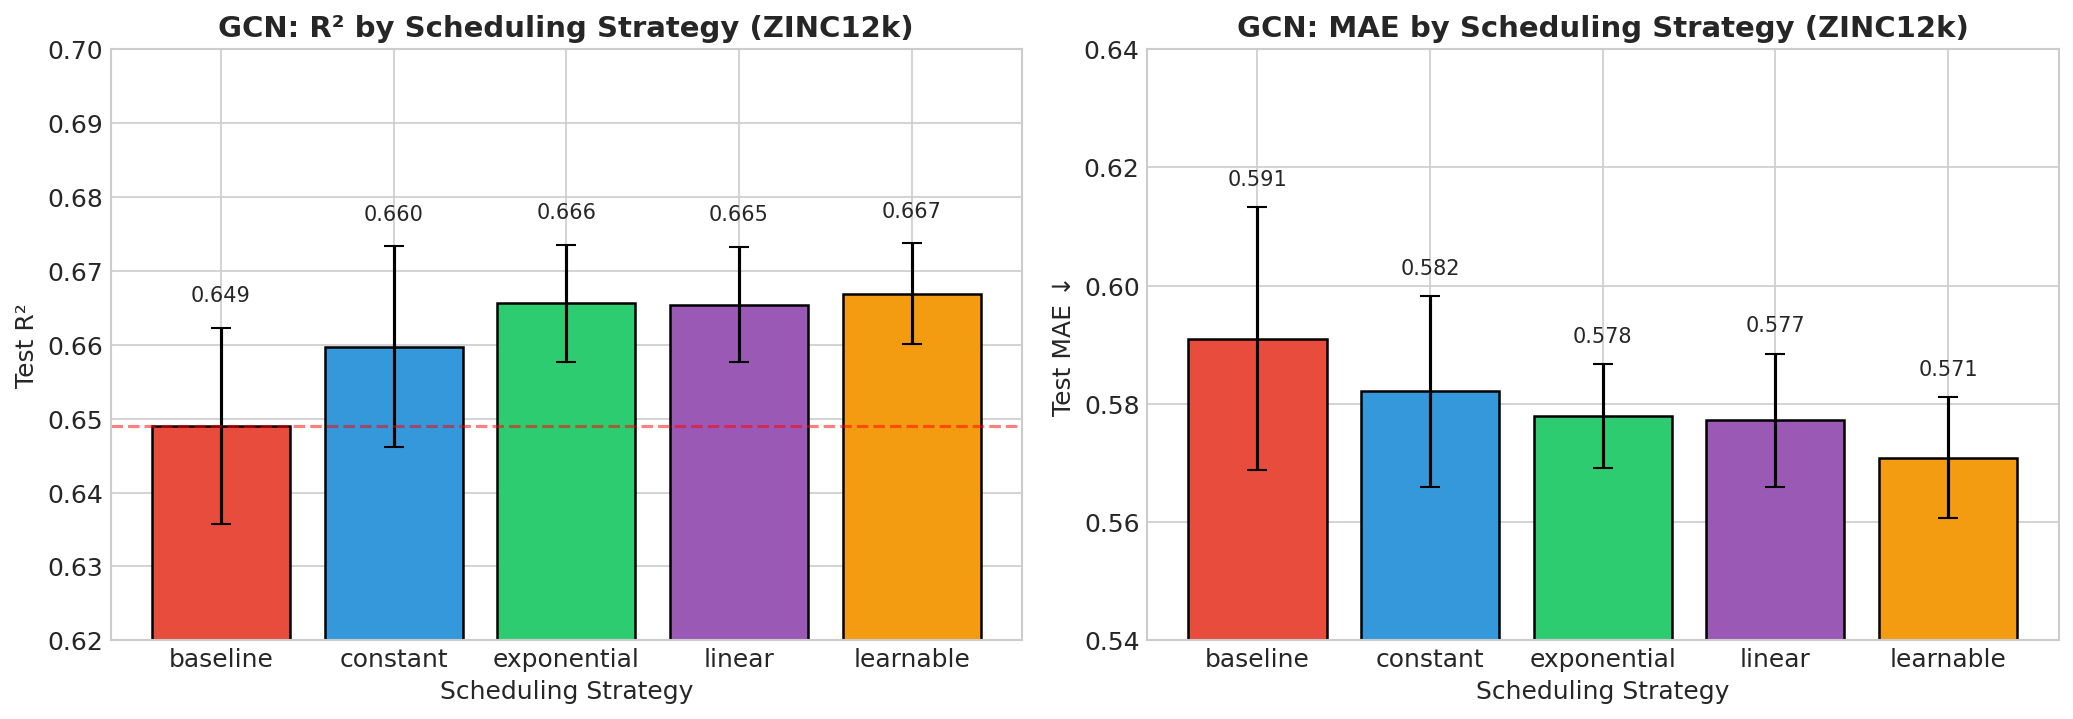
\includegraphics[width=0.95\textwidth]{plots/plot1_gcn_scheduling_comparison.png}
    \caption{Phase 1: GCN scheduling strategy comparison showing (left) Test $R^2$ and (right) Test MAE across 5 random seeds. Learnable scheduling achieves the best mean performance with lowest variance.}
    \label{fig:phase1}
\end{figure}

\begin{figure}[H]
    \centering
    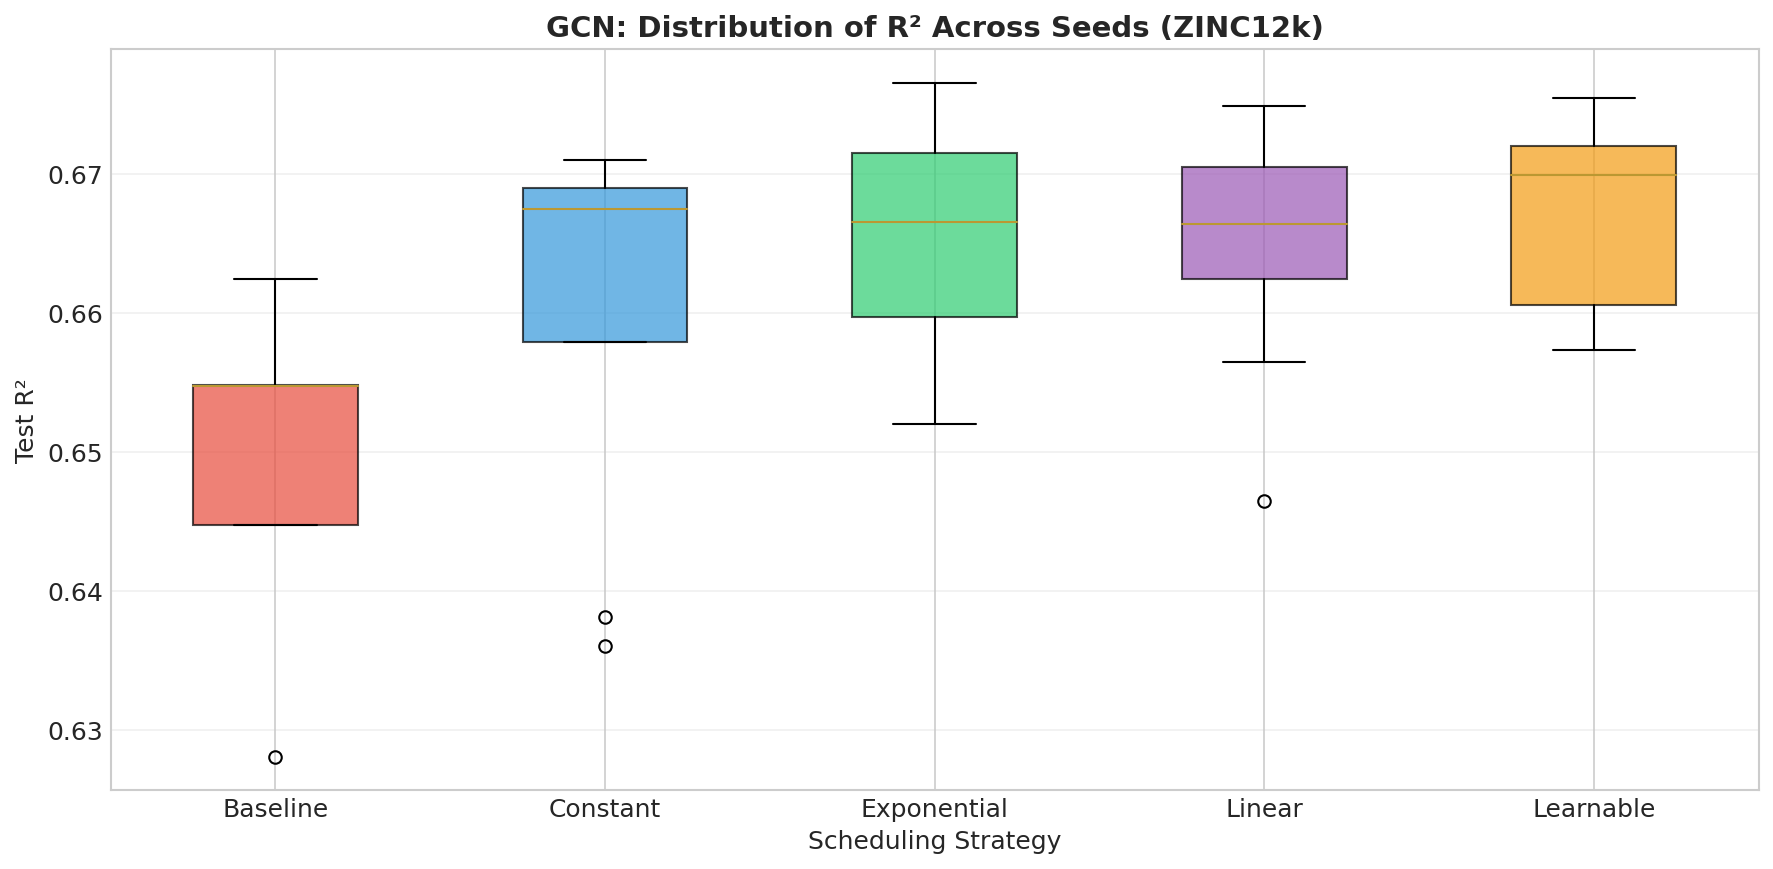
\includegraphics[width=0.7\textwidth]{plots/plot5_variance_boxplot.png}
    \caption{Distribution of Test $R^2$ across seeds for each scheduling strategy. Learnable scheduling shows the tightest distribution, indicating more consistent performance.}
    \label{fig:variance}
\end{figure}

\subsection{Phase 2: Architecture Comparison}

\begin{table}[H]
\centering
\caption{Phase 2: Architecture Comparison (Best Schedule per Model)}
\label{tab:phase2_summary}
\begin{tabular}{llcccc}
\toprule
\textbf{Model} & \textbf{Best Schedule} & \textbf{Test MAE} $\downarrow$ & \textbf{Test $R^2$} $\uparrow$ & \textbf{Epochs} & \textbf{Rank} \\
\midrule
\textbf{GIN} & Baseline & $\mathbf{0.407 \pm 0.009}$ & $\mathbf{0.838 \pm 0.004}$ & 227.6 & 1 \\
GIN & Constant & $0.429 \pm 0.040$ & $0.814 \pm 0.056$ & 215.4 & 2 \\
GCN & Learnable & $0.571 \pm 0.010$ & $0.667 \pm 0.007$ & 285.2 & 3 \\
GraphSAGE & Exponential & $0.604 \pm 0.011$ & $0.659 \pm 0.006$ & 194.0 & 4 \\
\bottomrule
\end{tabular}
\end{table}

\begin{table}[H]
\centering
\caption{Phase 2: Detailed Model $\times$ Schedule Breakdown}
\label{tab:phase2_detail}
\begin{tabular}{llccc}
\toprule
\textbf{Model} & \textbf{Schedule} & \textbf{Test MAE} & \textbf{Test $R^2$} & \textbf{$\Delta$ vs Baseline} \\
\midrule
\multirow{5}{*}{GIN} 
 & Baseline & $0.407 \pm 0.009$ & $\mathbf{0.838 \pm 0.004}$ & --- \\
 & Constant & $0.429 \pm 0.040$ & $0.814 \pm 0.056$ & $-2.9\%$ \\
 & Exponential & $0.513 \pm 0.011$ & $0.702 \pm 0.005$ & $-16.2\%$ \\
 & Linear & $0.513 \pm 0.019$ & $0.702 \pm 0.010$ & $-16.2\%$ \\
 & Learnable & $0.536 \pm 0.036$ & $0.686 \pm 0.021$ & $-18.1\%$ \\
\midrule
\multirow{5}{*}{GraphSAGE}
 & Baseline & $0.619 \pm 0.011$ & $0.647 \pm 0.007$ & --- \\
 & Constant & $0.608 \pm 0.011$ & $0.652 \pm 0.004$ & $+0.8\%$ \\
 & Exponential & $0.604 \pm 0.011$ & $\mathbf{0.659 \pm 0.006}$ & $+1.9\%$ \\
 & Linear & $0.604 \pm 0.012$ & $0.659 \pm 0.005$ & $+1.9\%$ \\
 & Learnable & $0.604 \pm 0.006$ & $0.653 \pm 0.004$ & $+0.9\%$ \\
\bottomrule
\end{tabular}
\end{table}

\begin{figure}[H]
    \centering
    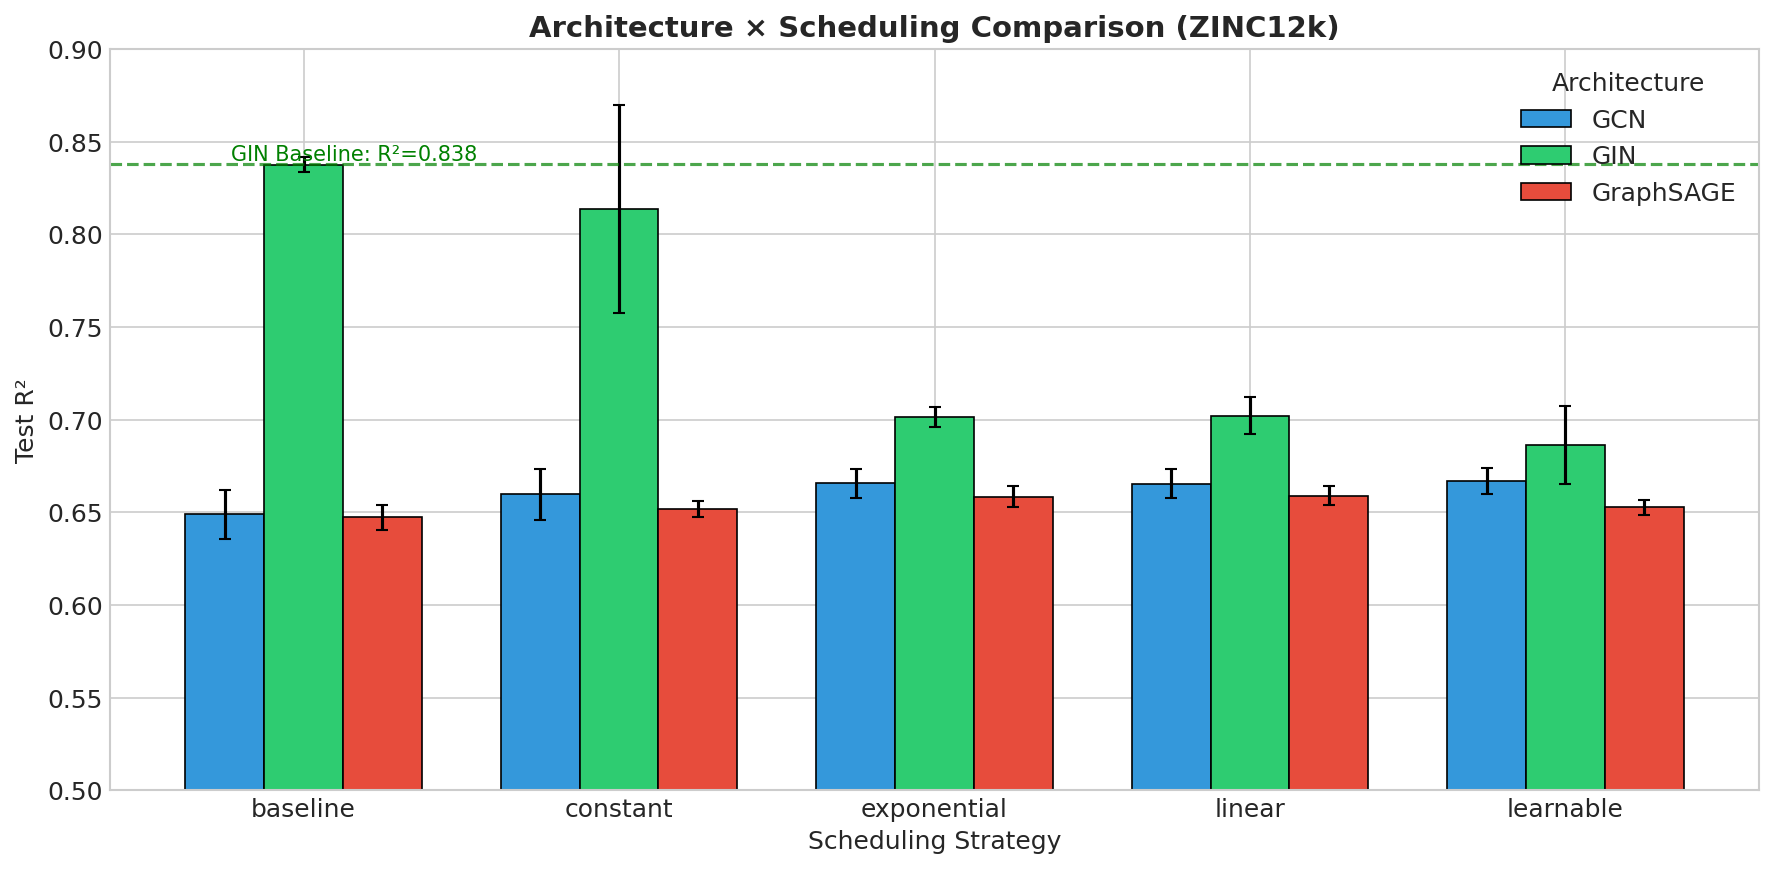
\includegraphics[width=0.95\textwidth]{plots/plot2_architecture_comparison.png}
    \caption{Architecture $\times$ Scheduling comparison. GIN baseline (leftmost green bar) dramatically outperforms all other configurations. Equivariance regularization helps GCN but hurts GIN.}
    \label{fig:architecture}
\end{figure}

\textbf{Critical Finding: Architecture Selection Dominates}

The most important finding from Phase 2 is that \textbf{architecture choice matters far more than scheduling strategy}:

\begin{itemize}
    \item \textbf{GIN baseline achieves $R^2 = 0.838$}, outperforming the best GCN configuration by \textbf{25.6\%} relative improvement
    \item \textbf{Equivariance regularization \textit{hurts} GIN performance} by up to 18\%, suggesting that GIN's inherent expressivity already captures the necessary structure
    \item For GraphSAGE, equivariance provides modest improvements (+1.9\%) similar to GCN
\end{itemize}

\begin{figure}[H]
    \centering
    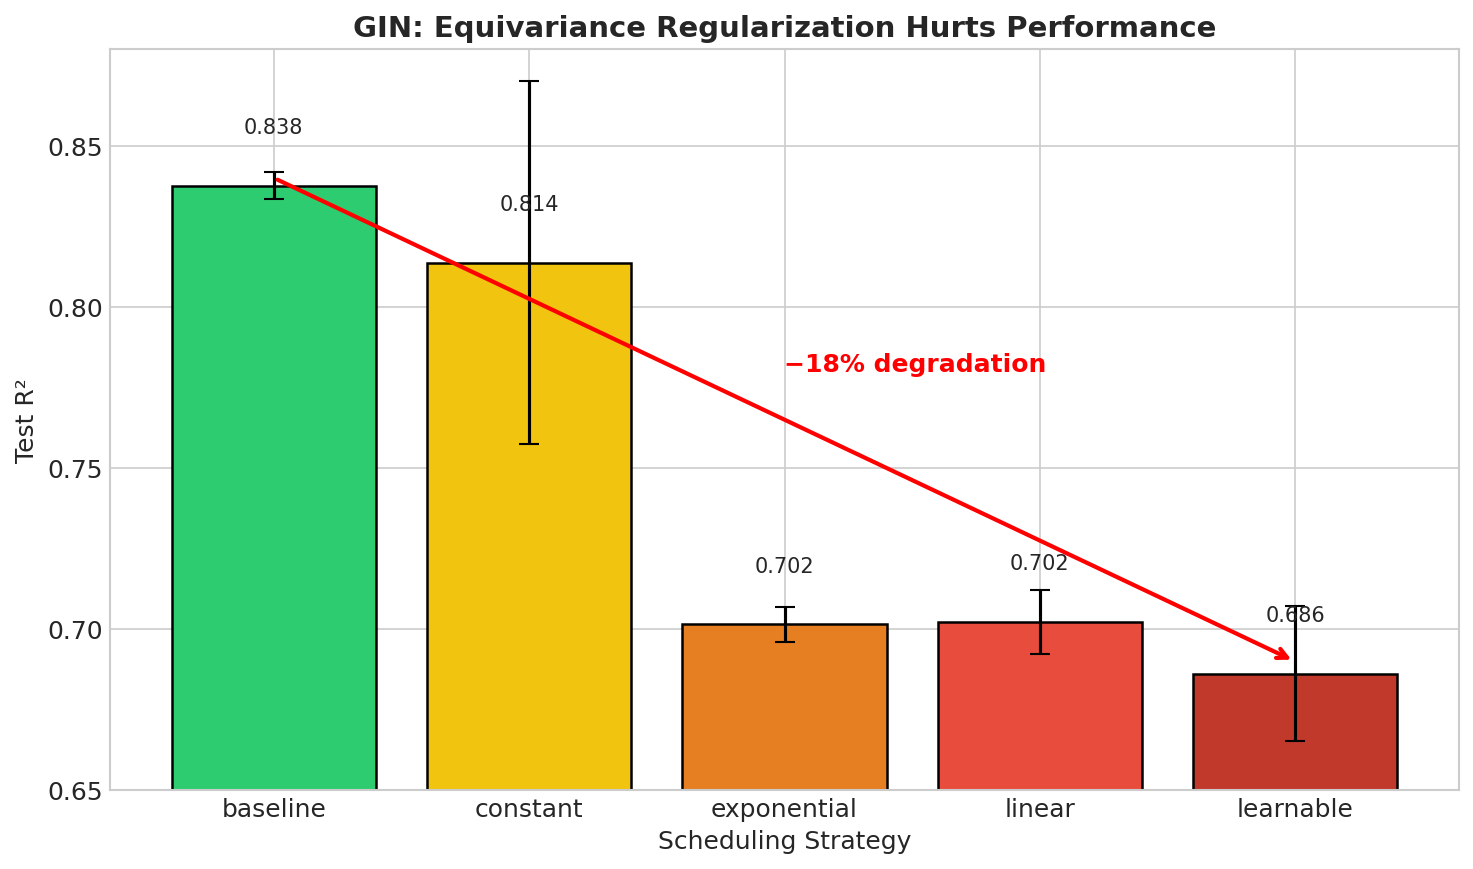
\includegraphics[width=0.8\textwidth]{plots/plot7_gin_equivariance_impact.png}
    \caption{GIN performance degradation with equivariance regularization. The baseline (no regularization) achieves $R^2 = 0.838$, while learnable scheduling drops to $R^2 = 0.686$---an 18\% degradation.}
    \label{fig:gin_impact}
\end{figure}

\subsection{Ablation Study: $\alpha_0$ and $\beta$ Sensitivity}

\begin{table}[H]
\centering
\caption{Ablation Study: $R^2$ by $\alpha_0 \times \beta$ Grid (GCN, 3 seeds each)}
\label{tab:ablation}
\begin{tabular}{l|cccc}
\toprule
\diagbox{$\alpha_0$}{$\beta$} & 0.0 & 0.1 & 0.3 & 0.5 \\
\midrule
0.0 & $0.640 \pm 0.015$ & --- & --- & --- \\
0.1 & --- & $0.641 \pm 0.015$ & $0.627 \pm 0.029$ & $0.635 \pm 0.025$ \\
0.5 & --- & $0.640 \pm 0.008$ & $0.640 \pm 0.007$ & $0.632 \pm 0.027$ \\
1.0 & --- & \textit{pending} & \textit{pending} & \textit{pending} \\
\bottomrule
\end{tabular}
\end{table}

\begin{figure}[H]
    \centering
    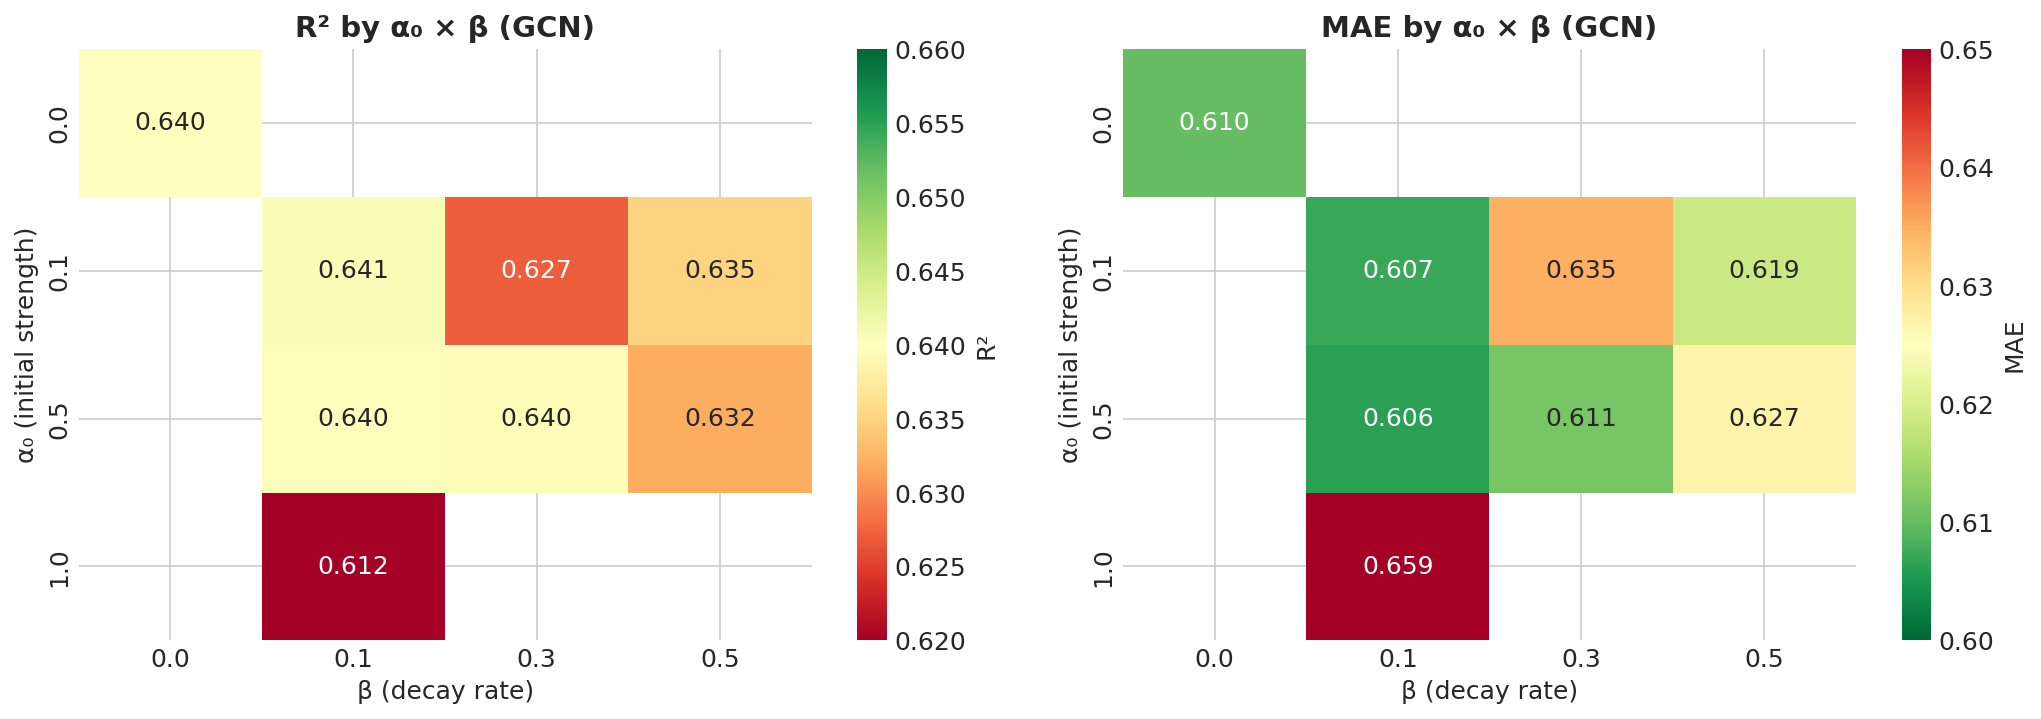
\includegraphics[width=0.95\textwidth]{plots/plot3_ablation_heatmap.png}
    \caption{Ablation study heatmaps for (left) $R^2$ and (right) MAE across the $\alpha_0 \times \beta$ parameter grid. Performance is relatively stable across the tested range.}
    \label{fig:ablation}
\end{figure}

\textbf{Preliminary Findings:}
\begin{itemize}
    \item Performance is \textbf{relatively stable} across the tested $\alpha_0$ and $\beta$ ranges
    \item Higher $\beta$ (faster decay) slightly reduces performance, suggesting gradual relaxation is preferred
    \item Best configuration so far: $\alpha_0 = 0.1$, $\beta = 0.1$ ($R^2 = 0.641$)
    \item Remaining experiments with $\alpha_0 = 1.0$ will complete the picture
\end{itemize}

\subsection{Depth Study}

\begin{table}[H]
\centering
\caption{Depth Study: Performance by Network Depth (GCN)}
\label{tab:depth}
\begin{tabular}{lccc}
\toprule
\textbf{Depth} & \textbf{Schedule} & \textbf{Test $R^2$} & \textbf{Test MAE} \\
\midrule
\multirow{3}{*}{4 layers}
 & Baseline & $0.645 \pm 0.018$ & $0.596 \pm 0.020$ \\
 & Exponential & $\mathbf{0.657 \pm 0.012}$ & $\mathbf{0.583 \pm 0.012}$ \\
 & Learnable & $0.652 \pm 0.013$ & $0.589 \pm 0.017$ \\
\midrule
\multirow{3}{*}{8 layers}
 & Baseline & $0.644 \pm 0.004$ & $0.600 \pm 0.005$ \\
 & Exponential & $0.648 \pm 0.012$ & $0.598 \pm 0.014$ \\
 & Learnable & $0.650$ (1 seed) & $0.594$ (1 seed) \\
\midrule
16 layers & \multicolumn{3}{c}{\textit{Experiments pending}} \\
\bottomrule
\end{tabular}
\end{table}

\begin{figure}[H]
    \centering
    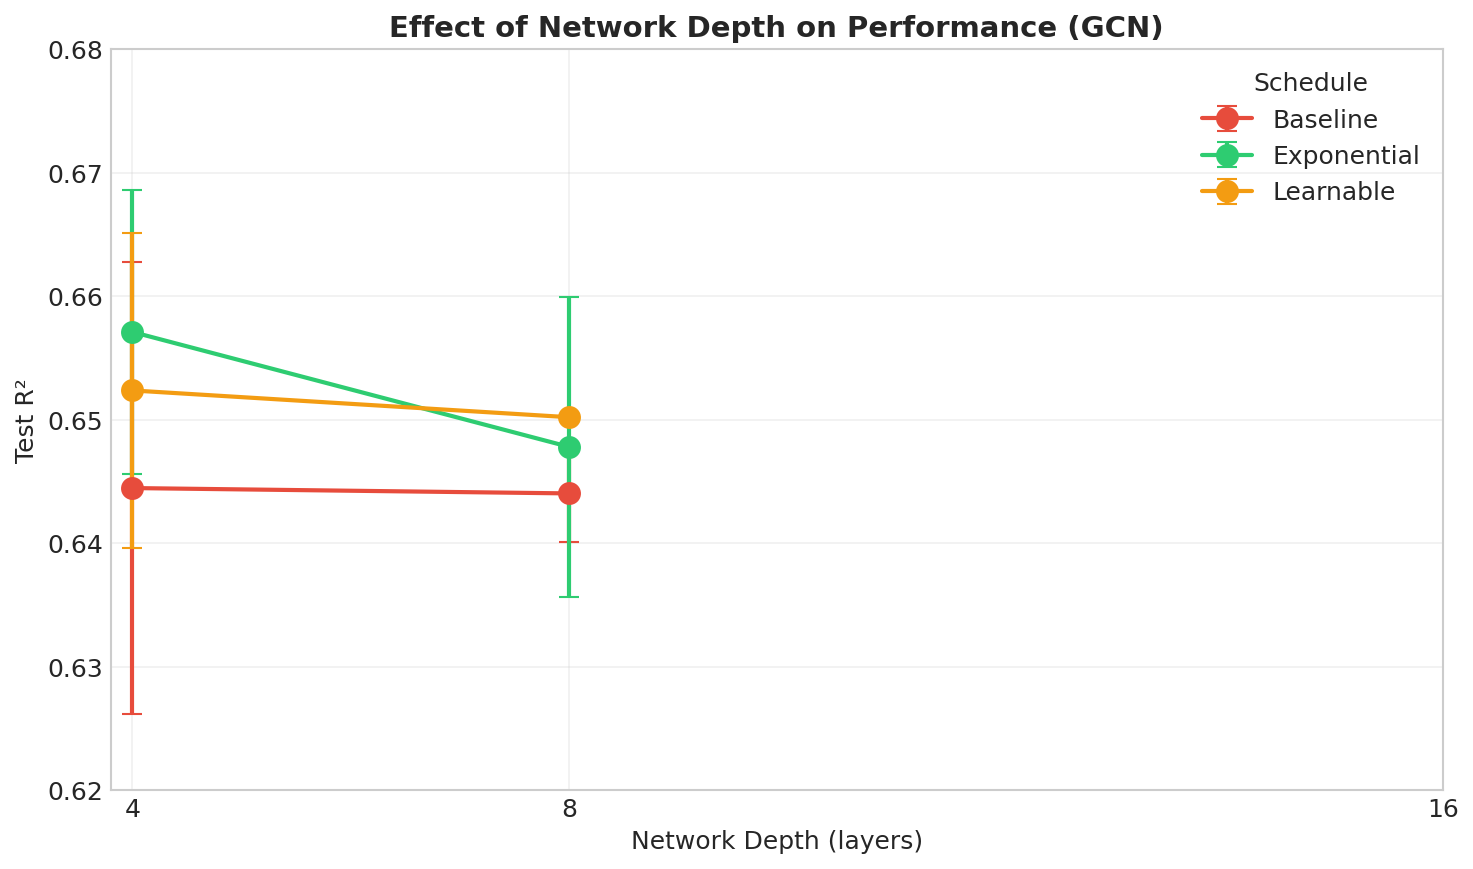
\includegraphics[width=0.8\textwidth]{plots/plot4_depth_study.png}
    \caption{Effect of network depth on performance. Shallow networks (4 layers) slightly outperform deeper ones, consistent with oversmoothing in GCN architectures.}
    \label{fig:depth}
\end{figure}

\textbf{Preliminary Findings:}
\begin{itemize}
    \item \textbf{Depth 4 slightly outperforms depth 8} for all scheduling strategies
    \item This is consistent with \textbf{oversmoothing} phenomena in GCN \cite{keriven2022oversmoothing}
    \item Equivariance regularization provides consistent benefits at both depths
    \item Depth 16 experiments pending---expected to show further degradation
\end{itemize}

\subsection{Summary of Best Results}

\begin{figure}[H]
    \centering
    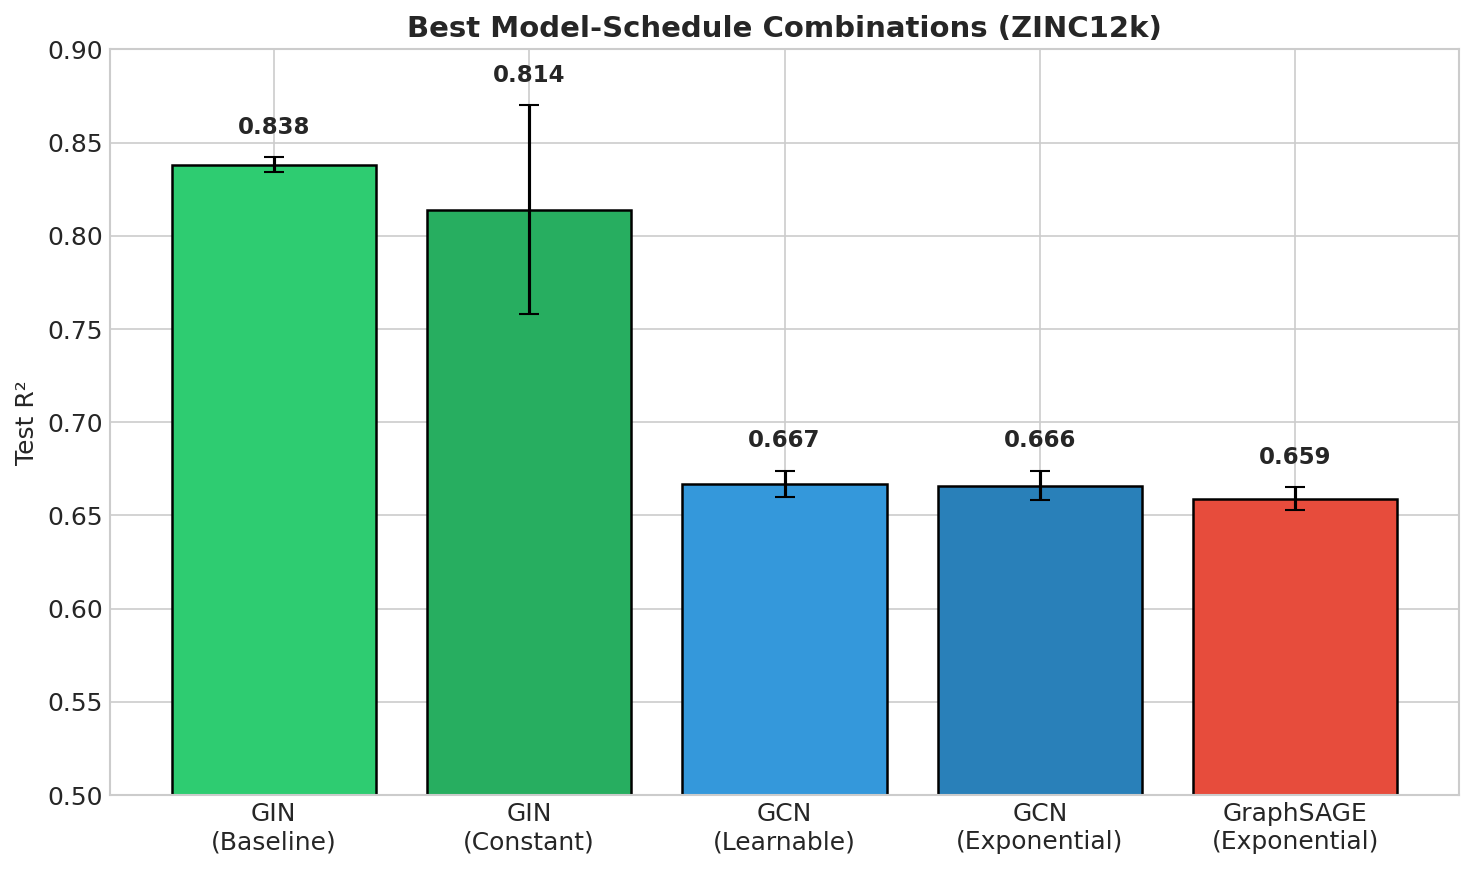
\includegraphics[width=0.85\textwidth]{plots/plot6_best_results_summary.png}
    \caption{Top 5 model-schedule configurations ranked by Test $R^2$. GIN baseline dominates, achieving $R^2 = 0.838$.}
    \label{fig:best}
\end{figure}

\begin{table}[H]
\centering
\caption{Top 5 Configurations Overall}
\label{tab:best}
\begin{tabular}{clcccc}
\toprule
\textbf{Rank} & \textbf{Configuration} & \textbf{Test $R^2$} & \textbf{Test MAE} & \textbf{Best Seed} \\
\midrule
1 & GIN + Baseline & $0.838 \pm 0.004$ & $0.407 \pm 0.009$ & 789 ($R^2=0.844$) \\
2 & GIN + Constant & $0.814 \pm 0.056$ & $0.429 \pm 0.040$ & 456 \\
3 & GIN + Exponential & $0.702 \pm 0.005$ & $0.513 \pm 0.011$ & 42 \\
4 & GCN + Learnable & $0.667 \pm 0.007$ & $0.571 \pm 0.010$ & 1000 ($R^2=0.677$) \\
5 & GCN + Exponential & $0.666 \pm 0.008$ & $0.578 \pm 0.009$ & 1000 ($R^2=0.677$) \\
\bottomrule
\end{tabular}
\end{table}

% ============ SECTION 7: DISCUSSION ============
\section{Discussion}

\subsection{Key Insights}

\subsubsection{Insight 1: Architecture Selection Dominates}

The most significant finding is that \textbf{choosing the right base architecture matters far more than the equivariance scheduling strategy}. GIN baseline achieves $R^2 = 0.838$, which is:
\begin{itemize}
    \item 25.6\% better than the best GCN configuration
    \item 27.1\% better than the best GraphSAGE configuration
    \item Better than \textit{any} equivariance-regularized GIN variant
\end{itemize}

This suggests that for practitioners, \textbf{starting with an expressive architecture} should be the first priority before considering equivariance regularization.

\subsubsection{Insight 2: Equivariance Benefits are Architecture-Dependent}

The benefit of relaxed equivariance depends strongly on the base model's expressivity:

\begin{itemize}
    \item \textbf{GCN (low expressivity)}: Equivariance helps (+2.8\% $R^2$)
    \item \textbf{GraphSAGE (medium expressivity)}: Equivariance helps modestly (+1.9\% $R^2$)
    \item \textbf{GIN (high expressivity)}: Equivariance \textit{hurts} ($-18\%$ $R^2$)
\end{itemize}

\textbf{Hypothesis}: GIN's MLP-based aggregation already captures sufficient structure, and adding equivariance constraints \textit{over-regularizes} the model, reducing its effective capacity.

\subsubsection{Insight 3: Learnable Scheduling is Most Robust for GCN}

For GCN, learnable $\alpha_l$ parameters:
\begin{itemize}
    \item Achieve the best mean performance ($R^2 = 0.667$)
    \item Have the \textbf{lowest variance} across seeds ($\pm 0.007$)
    \item Suggest that different layers benefit from different regularization strengths
\end{itemize}

\subsubsection{Insight 4: Computational Trade-offs}

Equivariance loss computation adds significant overhead:
\begin{itemize}
    \item Training time increases 2-3$\times$ due to additional forward passes for group sampling
    \item For GIN, this overhead is \textit{not justified} given performance degradation
    \item For GCN, the overhead may be acceptable given consistent improvements
\end{itemize}

\subsection{Limitations}

\begin{enumerate}
    \item \textbf{Single dataset}: All completed experiments use ZINC12k; generalization to other datasets (QM9, OGB) is pending
    
    \item \textbf{Permutation symmetry only}: Current experiments test only permutation equivariance; 3D geometric symmetries (SO(3), E(3)) are planned for Phase 3
    
    \item \textbf{Limited hyperparameter range}: Ablation study is incomplete; full $\alpha_0 \times \beta$ grid pending
    
    \item \textbf{Depth study incomplete}: Only 2 of 3 depths fully evaluated
    
    \item \textbf{No theoretical analysis}: Empirical findings need theoretical grounding
\end{enumerate}

\subsection{Practical Recommendations}

Based on our findings, we recommend:

\begin{enumerate}
    \item \textbf{Start with strong baselines}: Use GIN or other expressive architectures first
    
    \item \textbf{Match regularization to architecture}: Only apply equivariance regularization to less expressive models (GCN, simple GNNs)
    
    \item \textbf{Use learnable schedules when helpful}: For GCN-class architectures, learnable $\alpha_l$ provides best performance and lowest variance
    
    \item \textbf{Consider computational cost}: The 2-3$\times$ training overhead is only justified when equivariance provides clear benefits
\end{enumerate}

% ============ SECTION 8: ONGOING AND FUTURE WORK ============
\section{Ongoing and Future Work}

\subsection{Immediate Next Steps (Weeks 8-9)}

\begin{enumerate}
    \item \textbf{Complete Depth Study}
    \begin{itemize}
        \item Remaining: 11 experiments (depth 16, additional seeds)
        \item Expected: 1-2 days of computation
    \end{itemize}
    
    \item \textbf{Complete Ablation Study}
    \begin{itemize}
        \item Remaining: 17 experiments ($\alpha_0 = 1.0$ configurations)
        \item Expected: 2-3 days of computation
    \end{itemize}
    
    \item \textbf{Resume QM9 Experiments}
    \begin{itemize}
        \item Extend to 3D molecular data with geometric symmetries
        \item Test SO(3) and E(3) equivariance losses
    \end{itemize}
\end{enumerate}

\subsection{Extended Goals (Weeks 10-12)}

\begin{enumerate}
    \item \textbf{Graph Transformers}
    \begin{itemize}
        \item Extend depth-adaptive equivariance to Graphormer \cite{ying2021graphormer} and Equiformer \cite{liao2023equiformer}
        \item Compare with GNN baselines on same datasets
    \end{itemize}
    
    \item \textbf{Graph Rewiring Integration}
    \begin{itemize}
        \item Combine relaxed equivariance with spectral rewiring methods (FoSR, DiffWire)
        \item Test synergy for deep GNN architectures
    \end{itemize}
    
    \item \textbf{Bayesian $\alpha_l$ Optimization}
    \begin{itemize}
        \item Implement marginal likelihood optimization following \cite{vanderouderaa2023layerwise}
        \item Compare with gradient-based learnable $\alpha_l$
    \end{itemize}
    
    \item \textbf{Multi-task Benchmarks}
    \begin{itemize}
        \item Evaluate on PROMPT benchmark for protein multitask learning
        \item Test transferability of learned schedules across tasks
    \end{itemize}
\end{enumerate}

\subsection{Timeline}

\begin{table}[H]
\centering
\caption{Revised Project Timeline}
\label{tab:timeline}
\begin{tabular}{lll}
\toprule
\textbf{Week} & \textbf{Task} & \textbf{Status} \\
\midrule
1-2 & Literature review, formalization & \completed{Complete} \\
3-5 & Phase 1: GCN implementation and scheduling & \completed{Complete} \\
6-7 & Phase 2: Architecture comparison & \completed{Complete} \\
8 & Complete depth and ablation studies & \inprogress{In Progress} \\
9 & Resume QM9 experiments & Planned \\
10-11 & Graph transformers and rewiring & Planned \\
12 & Final analysis, write-up, submission & Planned \\
\bottomrule
\end{tabular}
\end{table}

% ============ SECTION 9: CONCLUSION ============
\section{Conclusion}

This progress report documents our systematic investigation of relaxed equivariance via multitask learning in Graph Neural Networks. Our key findings from 142 completed experiments are:

\begin{enumerate}
    \item \textbf{Architecture matters most}: GIN baseline ($R^2 = 0.838$) dramatically outperforms all other configurations, emphasizing that model selection is more important than regularization strategy
    
    \item \textbf{Equivariance benefits are architecture-dependent}: Relaxed equivariance helps less expressive models (GCN: +2.8\%) but hurts more expressive ones (GIN: $-18\%$)
    
    \item \textbf{Learnable scheduling is most robust}: For GCN, learnable $\alpha_l$ parameters achieve best performance with lowest variance
    
    \item \textbf{Depth-adaptive regularization shows promise}: Early results suggest layer-specific equivariance constraints can improve generalization for appropriate architectures
\end{enumerate}

The remaining experiments (depth study completion, ablation grid, QM9 dataset) will provide additional evidence and extend our findings to 3D geometric symmetries. Our reproducible experimental framework and comprehensive analysis establish a foundation for understanding when and how to apply relaxed equivariance in practice.

% ============ REFERENCES ============
\bibliographystyle{plainnat}
\begin{thebibliography}{20}

\bibitem[Bronstein et al.(2021)]{bronstein2021geometric}
Michael~M. Bronstein, Joan Bruna, Taco Cohen, and Petar Veličković.
\newblock Geometric deep learning: Grids, groups, graphs, geodesics, and gauges.
\newblock \emph{arXiv preprint arXiv:2104.13478}, 2021.

\bibitem[Elhag et al.(2024)]{elhag2024remul}
Ahmed Elhag, T.~Konstantin Rusch, Francesco Di~Giovanni, and Michael Bronstein.
\newblock Relaxed equivariance via multitask learning.
\newblock \emph{arXiv preprint arXiv:2410.17878}, 2024.

\bibitem[van~der Ouderaa et al.(2023)]{vanderouderaa2023layerwise}
Tycho van~der Ouderaa, Alexander Immer, and Mark van~der Wilk.
\newblock Learning layer-wise equivariances automatically using gradients.
\newblock In \emph{NeurIPS}, 2023.

\bibitem[Hofgard et al.(2024)]{hofgard2024relaxed}
Elyssa Hofgard et al.
\newblock Relaxed equivariant graph neural networks.
\newblock In \emph{ICML GRaM Workshop}, 2024.

\bibitem[Wang et al.(2022)]{wang2022approximate}
Rui Wang et al.
\newblock Approximately equivariant networks for imperfectly symmetric dynamics.
\newblock In \emph{ICML}, 2022.

\bibitem[Kipf and Welling(2017)]{kipf2017gcn}
Thomas~N. Kipf and Max Welling.
\newblock Semi-supervised classification with graph convolutional networks.
\newblock In \emph{ICLR}, 2017.

\bibitem[Xu et al.(2019)]{xu2019gin}
Keyulu Xu, Weihua Hu, Jure Leskovec, and Stefanie Jegelka.
\newblock How powerful are graph neural networks?
\newblock In \emph{ICLR}, 2019.

\bibitem[Hamilton et al.(2017)]{hamilton2017graphsage}
William~L. Hamilton, Rex Ying, and Jure Leskovec.
\newblock Inductive representation learning on large graphs.
\newblock In \emph{NeurIPS}, 2017.

\bibitem[Satorras et al.(2021)]{satorras2021egnn}
Victor~Garcia Satorras, Emiel Hoogeboom, and Max Welling.
\newblock E(n) equivariant graph neural networks.
\newblock In \emph{ICML}, 2021.

\bibitem[Liao and Smidt(2023)]{liao2023equiformer}
Yi-Lun Liao and Tess Smidt.
\newblock Equiformer: Equivariant graph attention transformer for 3d atomistic graphs.
\newblock In \emph{ICLR}, 2023.

\bibitem[Schütt et al.(2018)]{schutt2018schnet}
Kristof~T. Schütt et al.
\newblock SchNet: A continuous-filter convolutional neural network for modeling quantum interactions.
\newblock In \emph{NeurIPS}, 2018.

\bibitem[Schütt et al.(2021)]{schutt2021painn}
Kristof~T. Schütt, Oliver~T. Unke, and Michael Gastegger.
\newblock Equivariant message passing for the prediction of tensorial properties and molecular spectra.
\newblock In \emph{ICML}, 2021.

\bibitem[Keriven(2022)]{keriven2022oversmoothing}
Nicolas Keriven.
\newblock Not too little, not too much: A theoretical analysis of graph (over)smoothing.
\newblock In \emph{NeurIPS}, 2022.

\bibitem[Gilmer et al.(2017)]{gilmer2017mpnn}
Justin Gilmer et al.
\newblock Neural message passing for quantum chemistry.
\newblock In \emph{ICML}, 2017.

\bibitem[Dwivedi et al.(2023)]{dwivedi2023benchmarking}
Vijay~Prakash Dwivedi et al.
\newblock Benchmarking graph neural networks.
\newblock \emph{JMLR}, 2023.

\bibitem[Ying et al.(2021)]{ying2021graphormer}
Chengxuan Ying et al.
\newblock Do transformers really perform bad for graph representation?
\newblock In \emph{NeurIPS}, 2021.

\end{thebibliography}

% ============ APPENDIX ============
\appendix
\section{Appendix: Experimental Details}

\subsection{Complete Experiment Counts}

\begin{table}[H]
\centering
\caption{Detailed Experiment Breakdown}
\begin{tabular}{llccl}
\toprule
\textbf{Phase} & \textbf{Configuration} & \textbf{Completed} & \textbf{Total} & \textbf{Notes} \\
\midrule
Phase 1 & GCN $\times$ 5 schedules $\times$ seeds & 54 & 54 & Includes reruns \\
Phase 2 & GIN $\times$ 5 schedules $\times$ 5 seeds & 25 & 25 & Complete \\
Phase 2 & GraphSAGE $\times$ 5 schedules $\times$ 5 seeds & 25 & 25 & Complete \\
Ablation & $\alpha_0 \times \beta$ grid $\times$ 3 seeds & 22 & 39 & 56\% complete \\
Depth & Depth $\times$ schedule $\times$ 3 seeds & 16 & 27 & 59\% complete \\
Phase 3 & QM9 preliminary & 9 & 30+ & Paused \\
\midrule
\textbf{Total} & & \textbf{142} & \textbf{200+} & \\
\bottomrule
\end{tabular}
\end{table}

\subsection{Hyperparameter Settings}

\begin{table}[H]
\centering
\caption{Complete Hyperparameter Configuration}
\begin{tabular}{lll}
\toprule
\textbf{Category} & \textbf{Parameter} & \textbf{Value} \\
\midrule
\multirow{4}{*}{Architecture}
 & Hidden dimension & 64 \\
 & Number of layers & 4 (default), \{4, 8, 16\} (depth study) \\
 & Dropout rate & 0.5 \\
 & Activation & ReLU \\
\midrule
\multirow{5}{*}{Training}
 & Optimizer & Adam \\
 & Learning rate & 0.001 \\
 & LR scheduler & Cosine annealing \\
 & Batch size & 32 \\
 & Max epochs & 300 \\
 & Early stopping patience & 20 \\
\midrule
\multirow{4}{*}{Equivariance}
 & $\alpha_0$ & 1.0 (default), \{0.0, 0.1, 0.5, 1.0\} (ablation) \\
 & $\beta$ (exponential) & 0.1 (default), \{0.0, 0.1, 0.3, 0.5\} (ablation) \\
 & $\gamma$ (linear) & 0.1 \\
 & Symmetry group & Permutation ($S_n$) \\
 & Samples per batch & 3 \\
\midrule
\multirow{2}{*}{Reproducibility}
 & Random seeds & 42, 123, 456, 789, 1000 \\
 & PyTorch deterministic & True \\
\bottomrule
\end{tabular}
\end{table}

\subsection{Code Availability}

All code, configurations, and experimental logs are available at:
\begin{center}
\url{https://github.com/[repository]}
\end{center}

The repository includes:
\begin{itemize}
    \item \texttt{train.py}: Main training script with configurable equivariance losses
    \item \texttt{equivariance\_loss.py}: Implementation of layer-wise equivariance computation
    \item \texttt{schedulers.py}: Scheduling strategies (constant, exponential, linear, learnable)
    \item \texttt{config.py}: Experiment configuration management
    \item \texttt{generate\_plots.py}: Plotting scripts for all figures in this report
\end{itemize}

\end{document}